\documentclass[12pt]{article}
\usepackage[top=1in, bottom=1in, left=.75in, right=.75in]{geometry}
\usepackage{amsmath, enumerate}
\usepackage{fancyhdr}
\usepackage{graphicx, xcolor, setspace}
\usepackage{txfonts}
\usepackage{multicol,coordsys,pgfplots}
\usepackage[scaled=0.86]{helvet}
\renewcommand{\emph}[1]{\textsf{\textbf{#1}}}
\usepackage{anyfontsize}
% \usepackage{times}
% \usepackage[lf]{MinionPro}
\usepackage{tikz,pgfplots}
%\def\degC{{}^\circ{\rm C}}
\def\ra{\rightarrow}
\usetikzlibrary{calc,arrows.meta}
\usepackage[mathscr]{euscript}
\usepackage{tikz, tkz-euclide}
\usetikzlibrary{calc, through}
\usetikzlibrary{decorations.markings}
\usetikzlibrary{arrows, backgrounds}
\usetikzlibrary{positioning}
\usetikzlibrary{intersections}

\pgfplotsset{compat = newest}
\newcommand{\blank}[1]{\rule{#1}{0.75pt}}

\pgfplotsset{my style/.append style={axis x line=middle, axis y line=
middle, xlabel={$x$}, ylabel={$y$}}}

%axis equal

%yticklabels={,,} , xticklabels={,,}

% \setmainfont{Times}
% \def\sansfont{Lucida Grande Bold}
\parindent 0pt
\parskip 4pt
\pagestyle{fancy}
\fancyfoot[C]{\emph{\thepage}}
\fancyfoot[R]{v1}
\fancyhead[L]{\ifnum \value{page} > 1\relax\emph{Math F251X: Midterm 2}\fi}
\fancyhead[R]{\ifnum \value{page} > 1\relax\emph{Spring 2024}\fi}
\headheight 15pt
\renewcommand{\headrulewidth}{0pt}
\renewcommand{\footrulewidth}{0pt}
\let\ds\displaystyle
\def\continued{{\emph {Continued....}}}
\def\continuing{{\emph {Problem \arabic{probcount} continued....}}\par\vskip 4pt}


\newcounter{probcount}
\newcounter{subprobcount}
\newcommand{\thesubproblem}{\emph{\alph{subprobcount}.}}
\def\problem#1{\setcounter{subprobcount}{0}%
\addtocounter{probcount}{1}{\emph{\arabic{probcount}.\hskip 1em(#1)}}\par}
\def\subproblem#1{\par\hangindent=1em\hangafter=0{%
\addtocounter{subprobcount}{1}\thesubproblem\emph{#1}\hskip 1em}}
\def\probskip{\vskip 10pt}
\def\medprobskip{\vskip 2in}
\def\subprobskip{\vskip 45pt}
\def\bigprobskip{\vskip 4in}


\newenvironment{subproblems}{%
\begin{enumerate}%
\setcounter{enumi}{\value{subprobcount}}%
\renewcommand{\theenumi}{\emph{\alph{enumi}}}}%
{\setcounter{subprobcount}{\value{enumi}}\end{enumerate}}


\newcommand{\be}{\begin{enumerate}}
\newcommand{\ee}{\end{enumerate}}


\begin{document}
{\emph{\fontsize{26}{28}\selectfont Spring 2024 \hfill
%{\fontsize{32}{36}\selectfont Calculus 1: Midterm 1}
\hfill Math F251X}}

\begin{center}
{\emph{%\fontsize{26}{28}\selectfont Spring 2024 
%%\hfill
{\fontsize{32}{36}\selectfont Calculus 1: Midterm 2}
%%\hfill Math F251X}
}}
\end{center}

%\vskip 2cm
\strut\vtop{\halign{\emph#\hskip 0.5em\hfil&#\hbox to 2in{\hrulefill}\cr
\emph{\fontsize{18}{22}\selectfont Name:}&\cr
%\noalign{\vskip 10pt}
%\emph{\fontsize{18}{22}\selectfont Student Id:}&\cr
%\noalign{\vskip 10pt}
%\emph{\fontsize{18}{22}\selectfont Calculator Model:}&\cr
}}
\hfill
\vtop{\halign{\emph{\fontsize{18}{22}\selectfont #}\hfil& \emph{\fontsize{18}{22}\selectfont\hskip 0.5ex $\square$ #}\hfil\cr
Section: & 9:15am (James Gossell)\cr
\noalign{\vskip 4pt}
         & 11:45am (Mohamed Nouh)\cr
\noalign{\vskip 4pt}
         & async (Leah Berman)\cr}}

\vfill
{\fontsize{18}{22}\selectfont\emph{Rules:}}

\begin{itemize}
\item Partial credit may be awarded, but you must show your work.

\item You may have a single handwritten $3'' \times 5''$ notecard, both sides.

\item Calculators are {\bf not} allowed. 

\item Place a box around your  \fbox{FINAL ANSWER} to each question where appropriate.

\item Turn off anything that might go beep during the exam.

\end{itemize}

%If you need extra space, you can use the back sides of the pages.
%Please make it obvious  when you have done so.



Good luck!
\vfill
\def\emptybox{\hbox to 2em{\vrule height 16pt depth 8pt width 0pt\hfil}}
\def\tline{\noalign{\hrule}}
\centerline{\vbox{\offinterlineskip
{
\bf\sf\fontsize{18pt}{22pt}\selectfont
\hrule
\halign{
\vrule#&\strut\quad\hfil#\hfil\quad&\vrule#&\quad\hfil#\hfil\quad
&\vrule#&\quad\hfil#\hfil\quad&\vrule#\cr
height 3pt&\omit&&\omit&&\omit&\cr
&Problem&&Possible&&Score&\cr\tline
height 3pt&\omit&&\omit&&\omit&\cr
&1&&12&&\emptybox&\cr\tline
&2&&6&&\emptybox&\cr\tline
&3&&7&&\emptybox&\cr\tline
&4&&10&&\emptybox&\cr\tline
&5&&18&&\emptybox&\cr\tline
&6&&11&&\emptybox&\cr\tline
&7&&12&&\emptybox&\cr\tline
&8&&12&&\emptybox&\cr\tline
&9&&12&&\emptybox&\cr\tline \tline
&Extra Credit&&5&&\emptybox&\cr\tline
&Total&&100&&\emptybox&\cr
}\hrule}}}

\newpage
%\begin{enumerate}
%%%%

%\problem{16 points}
%\begin{subproblems}
%\item 
%\end{subproblems}



%\newpage
%%%%%%%%%%%% Optimization

\problem{12 points} 
\begin{minipage}[b]{.6\linewidth}
A rectangular storage container is to be constructed to have a fixed volume of 8 $\mathrm{m}^{3}$. Its bottom and sides are to be made of material that costs \$1 per square meter, while the top is constructed of material that costs \$5/square meter. The length of the base of the box is twice the width.
\end{minipage}
%
\hfill
%
\begin{minipage}{.2\linewidth}
\def\r{.4}
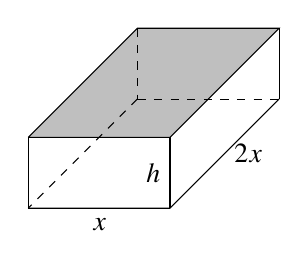
\begin{tikzpicture}[scale=.6]
\def\xx{3}
\def\hh{1.5}

%%y is up, z+ is out
\draw[black] (0,0,0) -- node[below]{$x$} (\xx, 0,0) -- node[right]{$2x$} (\xx,  0, - 2*\xx);
\draw[black] (0,0,0) -- (0, \hh, 0);
\draw[black] (\xx,0,0) -- node[left] {$h$} (\xx, \hh, 0);
\draw[black] (\xx,0,- 2*\xx) -- (\xx, \hh, - 2*\xx);
\filldraw[fill = gray!50] (0, \hh, 0) -- (\xx, \hh, 0) -- (\xx, \hh, - 2*\xx)--(0, \hh, - 2*\xx) -- (0, \hh, 0);
\draw[dashed] (0, \hh, - 2*\xx) -- (0,0,-2*\xx);
\draw[dashed] (0, 0, - 2*\xx) -- (\xx,0,-2*\xx);
\draw[dashed] (0, 0, - 2*\xx) -- (0,0,0);
\end{tikzpicture}
\end{minipage}

%\includegraphics[scale=0.6]{boxpic}
\begin{subproblems}
\item Write $h$ in terms of $x$ using the information in the problem.
\vspace{2cm}
\item Write a function for the \emph{total cost of the box} of the box in terms of the variable $x$.
\vspace{2cm}
\item %Determine which $x$ will {\bf maximize the volume} of the box. 
%Determine the exact value of $x$ that produces the box with the minimum cost.
Determine the \emph{dimensions} of the box with minimum cost.

Show your work, and use calculus to \emph{justify} that your answer is the minimum. Include units in your final answer. An answer with no clear justification or that does not use calculus techniques will not receive full credit.

\vfill

\vfill

\vfill

\emph{Dimensions:} width: \blank{1in} length: \blank{1in} height: \blank{1in}

\end{subproblems}

\newpage

\problem{6 points}
Suppose the side length of a cube is measured to be 5 cm, with a possible measurement error of $\pm \frac{1}{10}$ cm. 
\begin{subproblems}
\item Use linearization or differentials to estimate the possible error in the volume of the cube. 

\vspace{2in}

\item What is the relative error in the volume? %(Show some work.)
\vspace{1 cm}

\end{subproblems}

\problem{7 points} Find the absolute maximum and absolute minimum for the function %\[\displaystyle{ f(x) = 3x \ln(2x)}\] 
\[g(x) = (x - 2) (x + 3)^2 = x^3+4 x^2-3 x-18\]
on the interval $[-4,0].$ Justify how you know that you have found the absolute maximum and minimum. If there is no absolute maximum or minimum write ``none''. %Recall that $e \approx 2.71828$.
\vfill
Absolute maximum: $y =$ \hrulefill \ Absoute minimum: $y =$ \hrulefill
%%%%%%%%%%%%%%%%%%%%%%%%
\newpage
\problem{10 points} A small airplane is flying horizontally at an altitude of $3000$ m at a speed of $450$ km/hr = $125$ m/s.

At time $t = 0$ it passes above a camera on the ground that is pointed directly up. To keep the airplane in view, the angle of the camera changes. How fast is the angle $\theta$ (see diagram) changing when the plane has travelled $4000$ meters from the spot directly above the camera? Give your answer as an exact number, and include units.%How fast is the distance from
%the observer to the airplane increasing $30 \mathrm{s}$ later?



\begin{tikzpicture}
%\draw (0,0) node at (-0.7,-1) [anchor=north]{$1200 m$};
%\draw (0,0) node at (2,0.5) [anchor=north]{$x$};
\filldraw (0,0) -- (.15, .3) -- (-.15, .3) -- (0,0);

\draw[->,%decorate, decoration = snake
] (-2,-.1) node[left]{camera}--(-.1, .1);
\draw (0,0)
  -- node[left] {3000 m} (0,3)-- node[above] {$x$} (4,3) node[right]{airplane $\to$}
  -- cycle;
 \draw (.4,.3) arc   (30:90:.5) ;
 
 \node at (60:.8) {$\theta$};

\end{tikzpicture}



%%%%%%%%%%%%%%%%%%%%%%%%%%
\newpage
%%%%%%%%%%%%%%%%%%%%%%%%%%%
\problem{18 points} 
Answer the questions below about the function $\ds f(x)=\frac{45x^4-1584x^2}{440\sqrt[3]{x}}$. It is a fact that after simplification, \[ \quad f'(x)=\frac{3x^3-48x}{8\sqrt[3]{x}}, \quad \text{ and }  f''(x)=\frac{x^2-4}{\sqrt[3]{x}}\]
You must show your work and justify your conclusion with a few words or a computation. Make sure someone else can follow your work.
\begin{subproblems}
\item What is the domain of $f(x)$? (use interval notation) \hrulefill
	\item Determine the intervals where $f$ is \emph{increasing} and where $f$ is \emph{decreasing}. Show your work.
	\vfill
	
	\vfill
	
	Increasing: \hrulefill Decreasing:\hrulefill	(If none write ``none''.)
	
	\item Fill in the blanks: $f(x)$ has a local maximum at $x = $ \blank{1in}  and a local minimum at $x = \blank{1in} $. (If none, write ``none''.)
	
%	\continued
%	\newpage
	
%	\continuing
	
%	From the previous page, \[ f(x)=\frac{45x^4-1584x^2}{440\sqrt[3]{x}},    \quad f'(x)=\frac{3x^3-48x}{8\sqrt[3]{x}}, \quad \text{ and }  f''(x)=\frac{x^2-4}{\sqrt[3]{x}}\]


	\item Find all intervals where $f$ is \emph{concave up} and where $f$ is \emph{concave down}. Show your work.
	\vfill

	Concave up: \hrulefill Concave down:\hrulefill	(If none write ``none''.)
	
	\item Fill in the blanks: $f(x)$ has (an) inflection point(s) at $x =$ \blank{1in}. (If none, write ``none''.)
	
%	\item \textcolor{red}{ Do we want to ask anything about an asymptote at 0?}

\end{subproblems}

\newpage

\problem{11 points} \emph{Sketch} a graph of a function $h(x)$ that satisfies all of the following properties.

After drawing the graph:
\begin{itemize}
\item \emph{Label} on the graph the following things, if they exist, by drawing a point on the graph and labeling: any local maximums by writing  \textsf{LOCAL MAX}, local minimums by writing \textsf{LOCAL MIN}, inflection points by writing \textsf{IP} 
\item Draw any horizontal and vertical asymptotes with dashed lines and \emph{label} them with their equation.
\item Mark any important $x$-values and $y$-values on the $x$- and $y$-axes.
\end{itemize}


\emph{Properties:}
%\begin{multicols}{2}
%\begin{itemize}
%\item The domain of $h(x)$ is $(-\infty, 2)\cup(2, \infty)$.
%\item $h(0)=2$.
%\item $h'(x) > 0$ when $x<0$.
%\item $h'(x) < 0$ when $0<x<2$ and when $x>2$.
%\columnbreak
%\item $h''(x) > 0$ when $x < -2$ or $x > 2$.
%\item $h''(x) < 0$ when $-2 < x < 2$
%\item $\ds \lim_{x \to -\infty} h(x) = -2$
%\item $\ds \lim_{x \to \infty} h(x) = 1$
%\end{itemize}
%\end{multicols}

\begin{multicols}{2}
\begin{itemize}
\item The domain of $h(x)$ is $(-\infty, \infty)$.
\item $h(0)=2$.
\item $h'(x) > 0$ when $x<0$.
\item $h'(x) < 0$ when $x>0$.
\columnbreak
\item $h''(x) > 0$ when $x < -2$ or $x > 2$.
\item $h''(x) < 0$ when $-2 < x < 2$
\item $\ds \lim_{x \to -\infty} h(x) = -2$
\item $\ds \lim_{x \to \infty} h(x) = 1$
\end{itemize}
\end{multicols}

\begin{tikzpicture}
\draw[<->] (-8,0) --  (8,0);
\draw[<->] (0,4) -- (0,-4);
\end{tikzpicture}

\newpage



\problem{12 points} Evaluate the following limits. \emph{Show your work}, uncluding appropriate use of limit notation. If you use L'H\^opital's rule, you must indicate where you are using it by writing $\stackrel{H}{=}$ or $\stackrel{L'H}{=}$ or something similar. Use $\infty$ or $-\infty$ where appropriate, and if the limit does not exist, write {\sf DNE} and provide a justification.
\begin{subproblems}
\item $\displaystyle{\lim_{x\to 4} \frac{\ln(x-3)}{\sqrt{x}-2}}$
\vfill
\item $\ds \lim_{x \rightarrow 0} \frac{x^3-x^2}{3\cos x - 3}$
\vfill
\item $\ds \lim_{x \rightarrow \infty} \frac{e^{-x}+2}{\sec\left(\frac{1}{x}\right)}$
\vfill
\item $\ds \lim_{x \rightarrow \infty} \frac{12x^{10}+ 8x^{2} - 2}{7x^{9} + 11x^{4} + 6}$ 
\vfill
\end{subproblems}

\newpage


%%%%%%%%%%%%%%%%%%%%%%%%%%%%%%%%%%%%

\problem{12 points} A portion of the piecewise-linear function \[f(x) = \begin{cases} 
-x&\quad x\leq 3\\
\frac{3}{2}(x-5) &\quad x > 3
\end{cases} \]
is graphed below.

\begin{center}
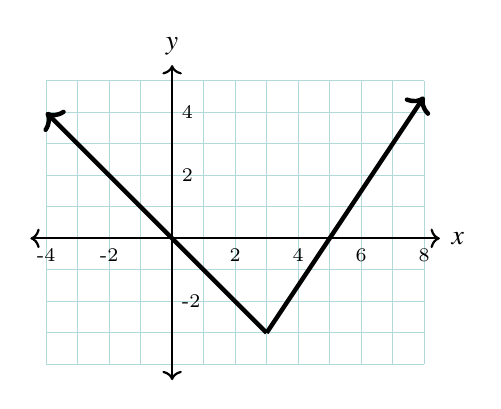
\begin{tikzpicture}[scale = .4]
%cubic
%\begin{axis}[xscale = 1, yscale = 1, thick, my style, xtick={-2,2,4,...,10}, ytick={-1,1,2,3,4},xmin=-5, xmax=10, ymin=-5, ymax=6, minor y tick num=1, minor x tick num=1, 
%mark size=3.0pt, grid = major, ]
%%\addplot[ultra thick, -,domain=-4:-2, samples=100, <-]coordinates {(-4,-2)(-2,2)};
%\addplot[ultra thick, domain=-5:5, samples=100, ,]{sqrt(25-x^2)};
%\addplot[ultra thick, ->,domain=5:9, samples=100]{-1/2*(x-5)};
%\end{axis}

\draw[help lines] (-4, -4) grid (8, 5);
\draw[thick,<->] (-4.5,0) -- (8.5,0) node[right] {$x$};
\draw[thick,<->] (0,-4.5) -- (0,5.5) node[above] {$y$};
\draw[ultra thick, ->] (3,-3) -- (8,3/2*8-3/2*5);
\draw[ultra thick, <-] (-4,4) -- (3,-3);
%\draw[ultra thick] (5,0) arc (0:180:5);
\foreach \i in { -4,-2,2,4,6,8} {\path  (\i,0)node[below, font = \scriptsize] {\i};}
\foreach \i in {-2,2,4} {\path  (0, \i)node[right, font = \scriptsize] {\i};}

\end{tikzpicture}
\end{center}


\begin{subproblems}
\item We want to approximate $\ds \int_{-2}^{7} f(x) \ dx$ using three left-hand rectangles.

\begin{enumerate}[i.]
%\begin{subproblems}
\item \emph{Draw} the three \emph{left-hand} rectangles on the graph. Lightly shade them in. Make sure I can tell where your rectangles are and try to be reasonably precise.
\bigskip

\item Now \emph{approximate} $\ds \int_{-2}^{7} f(x) \ dx$ using the  three \emph{left-hand} rectangles. (Your answer should be a number.) Show some work.
\vfill

%\end{subproblems}
\end{enumerate}
\item Use geometry to compute $\ds \int_{-2}^{7} f(x) \ dx$ exactly. Show your work.
%\vfill

\hfill 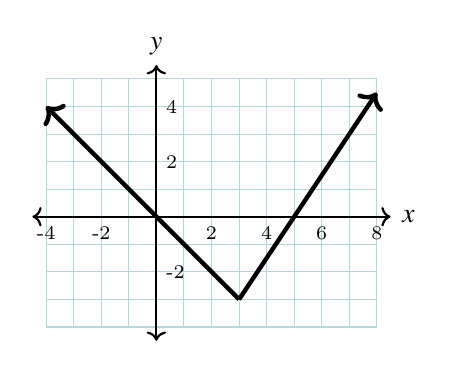
\begin{tikzpicture}[scale = .35]
%cubic
%\begin{axis}[xscale = 1, yscale = 1, thick, my style, xtick={-2,2,4,...,10}, ytick={-1,1,2,3,4},xmin=-5, xmax=10, ymin=-5, ymax=6, minor y tick num=1, minor x tick num=1, 
%mark size=3.0pt, grid = major, ]
%%\addplot[ultra thick, -,domain=-4:-2, samples=100, <-]coordinates {(-4,-2)(-2,2)};
%\addplot[ultra thick, domain=-5:5, samples=100, ,]{sqrt(25-x^2)};
%\addplot[ultra thick, ->,domain=5:9, samples=100]{-1/2*(x-5)};
%\end{axis}

\draw[help lines] (-4, -4) grid (8, 5);
\draw[thick,<->] (-4.5,0) -- (8.5,0) node[right] {$x$};
\draw[thick,<->] (0,-4.5) -- (0,5.5) node[above] {$y$};
\draw[ultra thick, ->] (3,-3) -- (8,3/2*8-3/2*5);
\draw[ultra thick, <-] (-4,4) -- (3,-3);
%\draw[ultra thick] (5,0) arc (0:180:5);
\foreach \i in { -4,-2,2,4,6,8} {\path  (\i,0)node[below, font = \scriptsize] {\i};}
\foreach \i in {-2,2,4} {\path  (0, \i)node[right, font = \scriptsize] {\i};}

\end{tikzpicture}

	\end{subproblems}


\newpage


\problem{12 points}Answer the following, showing work where necessary.

\begin{subproblems}


	\item $\displaystyle{ \int 4x - (\sec x)^{2}\ dx} \quad$ (give the most generic answer)

	\vfill
	
		\item $\displaystyle{ \int \frac{x^4-3x^2+5}{x^4} \ dx} \quad$ (give the most generic answer)
	\vfill


	\item The \emph{velocity} $v(t)$ of a particle is given by the function
	\[ v(t) = \sin(t) - \cos(t)\]
	and it has a position function $s(t)$. At time $t = 0$, $s(0) = 1$. Determine the  position function $s(t)$.
	\vfill

\end{subproblems}

\newpage


\newpage

%\end{enumerate}
%%%%%%%%%%%%%%%%%%%%%%%%%%%

\fbox{Extra Credit} (5 points)
The growth multiplier over a year for a savings account with an interest rate of $10\%$ compounded $x$ times per year is given by \[G(x) = \left(1+\frac{0.1}{x}\right)^x.\] 

For example, $G(1)=1.1$ means that you will multiply your money by $1.1$ if interest is compounded once per year. $G(2)=1.1025$ means that you will multiply your money by $1.1025$ if interest is compounded twice per year.\\

Calculate $\displaystyle \lim_{x \rightarrow \infty} G(x)$. What does this value mean in the context of the problem?

\end{document}

%%%%ENDDOCUMENT


